% !TEX encoding = IsoLatin 

% Affinch� gli accenti vengano accettati, assicurati che la codifica di questo file
% sia ISO 8859-1

% PER OTTENERE IL PDF, digitare da terminale
% ./makepdfplease
% 
\chapter[Valutazione dei risultati][]{5. Valutazione dei risultati}

Dopo l'implementazione dei due prototipi, possiamo introdurre la loro valutazione con l'uso della classe Scorer della libreria SpaCy.
La terminologia Scorer proviene dal mondo del Machine Learning ed indica l'affidabilit� della predizione di una data entit� in termini di \textbf{precision}, \textbf{recall} e \textbf{accuracy}.

\section{Scorer Class}
Lo Scorer � la classe fornita da SpaCy per valutare le performance di un modello annotatore per ogni singola entit� basandosi sulle 
annotazioni prodotte da tale modello.
Lo Scorer richiede all'utente della libreria di avere a disposizione l'output del modello annotatore e le gold annotations della Ground Truth.
Per ogni annotazione si crea un oggetto spacy.Span e si crea una lista di Span, che chiameremo labelled\_entities\_span\_list; si potr� poi utilizzare la lista di gold annotations per creare il relativo \textbf{item} che descrive l'annotazione di un documento:

\begin{lstlisting}[language=Python, caption=Esempio di item]
item = Example.from_dict(labelled_entities_span_list, 
                         {"entities": [[start_offset, end_offset, word]
                                      for [start_offset, end_offset, word]
                                      in gold_annots]})
\end{lstlisting}

Si crea un Example per ogni documento annotato e si pongono gli item in una \textbf{item\_list}.
Tutti i dati annotati dal modello annotatore sono ora nella item list ed � dunque possibile invocare 
il task di score vero e proprio:
\begin{lstlisting}[language=Python]
    scores = scorer.score(item_list)
\end{lstlisting}

\section{Confronto tra i due approcci}
Nella tabella scores-comparisons.pdf riporta i valori di Precision, Recall e Accuracy ottenuti per ogni entit� contemplata nel task di 
classificazione.


%allora\includegraphics[width=16cm, height=30cm,page=1]{scores-comparisons.pdf} %width=, height=, page=,
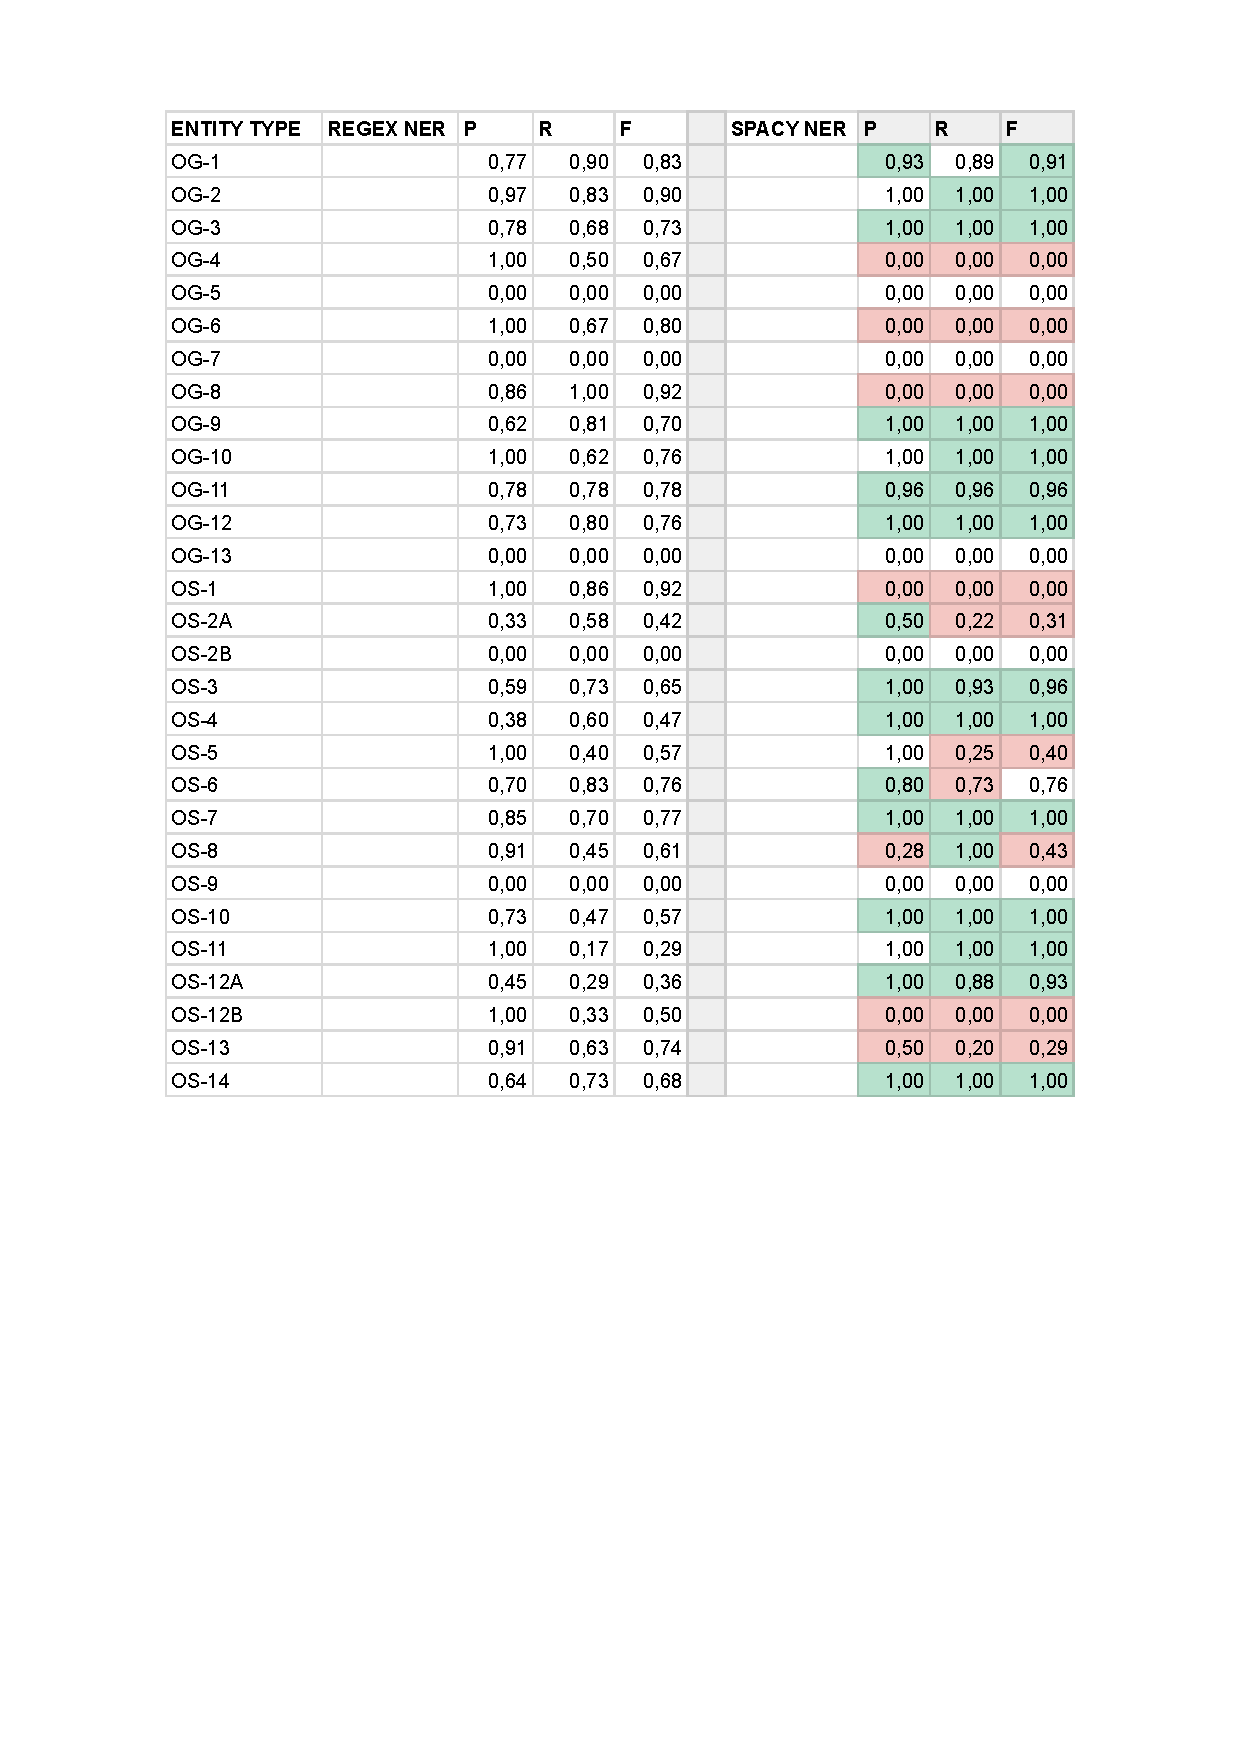
\includegraphics[trim=0 300 0 0, clip, width=\textwidth,height=\textheight,keepaspectratio, page=1]{confronti.pdf} 
\captionof{figure}{confronto tra l'approccio regex(sinistra) e NN(destra)}
Si pu� facilmente notare come molte entit� di tipo \textbf{Categoria} vedono valori di precision recall e accuracy migliori nell'approccio Machine Learning; questo miglioramento si rivela significativo in circa il 60\% delle entit� categoria.
Nel restante 40\% delle categorie si registra un peggioramento delle performance del Machine Learning, che in pochi ma significativi casi abbatte a zero le score.
Questo pu� essere dovuto alla mancanza di esempi numerosi per tutte le entit�: 
ci� porterebbe il modello a funzionare molto bene nel riconoscere le entit� ben rappresentate dalla ground truth,
ma anche a funzionare peggio per tutte le entit� meno note.
Le regex invece, fornendo a priori i pattern di ogni entit�, non soffrono della mancanza di esempi. 
\section{Conclusioni}
Come sottolineato precedentemente, l'approccio NER con regex non ha grandi margini di miglioramento dell'accuratezza:
in sintesi � un approccio rigido, che in caso di inclusione di nuovi pattern testuali 
richiederebbe la continua modifica di una regex in forme sempre pi� complesse, risolvendosi in
problemi di manutenzione, di testing, di leggibilit� e talvolta di sicurezza.
Nel caso del Machine Learning un task di \acrfull{named-entity-recognition} pu� avere risultati migliori delle regex, 
ma pu� soffrire di carenza di esempi per alcune entit�.
Su questa base si potrebbe proporre l'uso combinato degli output di entrambi i modelli: in particolare,
si potrebbe ricorrere al modello regex per le entit� meno assimilate dal modello \acrfull{machine-learning}
, preferendo invece quest'ultimo
per le entit� su cui gli score descrivono prestazioni migliori.


